\documentclass{article}

% if you need to pass options to natbib, use, e.g.:
% \PassOptionsToPackage{numbers, compress}{natbib}
% before loading nips_2018

% ready for submission
\usepackage{nips_2018}

% to compile a preprint version, e.g., for submission to arXiv, add
% add the [preprint] option:
% \usepackage[preprint]{nips_2018}

% to compile a camera-ready version, add the [final] option, e.g.:
% \usepackage[final]{nips_2018}

% to avoid loading the natbib package, add option nonatbib:
% \usepackage[nonatbib]{nips_2018}

\usepackage[utf8]{inputenc} % allow utf-8 input
\usepackage[T1]{fontenc}    % use 8-bit T1 fonts
\usepackage{hyperref}       % hyperlinks
\usepackage{url}            % simple URL typesetting
\usepackage{booktabs}       % professional-quality tables
\usepackage{amsfonts}       % blackboard math symbols
\usepackage{nicefrac}       % compact symbols for 1/2, etc.
\usepackage{microtype}      % microtypography

\usepackage{amsmath}
\usepackage{amssymb}

\newcommand{\etal}{\textit{et al}.}
\newcommand{\ie}{\textit{i}.\textit{e}.}
\newcommand{\eg}{\textit{e}.\textit{g}.}

\newcommand{\MW}[1]{{\color{blue} {\bf (MW: #1)}}}
\newcommand{\AY}[1]{{\color{purple} {\bf (AY: #1)}}}

\newcommand{\newl}{\newline}
\newcommand{\bm}{\mathbf}

\newcommand{\bW}{\bm{W}}
\newcommand{\bV}{\bm{V}}
\newcommand{\bD}{\bm{D}}

\title{Adaptive Phase Filter Networks: 
\newline Supplementary Materials}

% The \author macro works with any number of authors. There are two
% commands used to separate the names and addresses of multiple
% authors: \And and \AND.
%
% Using \And between authors leaves it to LaTeX to determine where to
% break the lines. Using \AND forces a line break at that point. So,
% if LaTeX puts 3 of 4 authors names on the first line, and the last
% on the second line, try using \AND instead of \And before the third
% author name.

\author{
  David S.~Hippocampus\thanks{Use footnote for providing further
    information about author (webpage, alternative
    address)---\emph{not} for acknowledging funding agencies.} \\
  Department of Computer Science\\
  Cranberry-Lemon University\\
  Pittsburgh, PA 15213 \\
  \texttt{hippo@cs.cranberry-lemon.edu} \\
  %% examples of more authors
  %% \And
  %% Coauthor \\
  %% Affiliation \\
  %% Address \\
  %% \texttt{email} \\
  %% \AND
  %% Coauthor \\
  %% Affiliation \\
  %% Address \\
  %% \texttt{email} \\
  %% \And
  %% Coauthor \\
  %% Affiliation \\
  %% Address \\
  %% \texttt{email} \\
  %% \And
  %% Coauthor \\
  %% Affiliation \\
  %% Address \\
  %% \texttt{email} \\
}

\begin{document}
% \nipsfinalcopy is no longer used

\maketitle

\begin{abstract}
  The abstract paragraph should be indented \nicefrac{1}{2}~inch
  (3~picas) on both the left- and right-hand margins. Use 10~point
  type, with a vertical spacing (leading) of 11~points.  The word
  \textbf{Abstract} must be centered, bold, and in point size 12. Two
  line spaces precede the abstract. The abstract must be limited to
  one paragraph.
\end{abstract}


\subsection{Model stability}
\MW{This should go into the appendix, no?}
For $\mathbf{z} \neq \mathbf{1}$ derivatives will distribute over a sum, forming a constant error carrousel as described in \cite{Hochreiter}. Choosing the gate bias to be large we initially have $\mathbf{z} \approx \mathbf{1}$ and a situation similar to \cite{Arjovsky} considering their formulation, while taking into account the added reset gate we obtain: 
\begin{align}
\frac{\partial C}{\partial \mathbf{h}_{t}} &= \frac{\partial C}{\partial \mathbf{h}_T}\frac{\partial 
                                              \mathbf{h}_T}{\partial \mathbf{h}_t}, 
                                     \label{eq:peep_cost} \\
                                  &= \frac{\partial C}{\partial \mathbf{h}_T}\prod_{k=t}^{T-1}\frac{\partial \mathbf{h}_{k+1}}{\partial \mathbf{h}_k}, \\
                                  &= \frac{\partial C}{\partial \mathbf{h}_T}\prod_{k=t}^{T-1}\mathbf{U}_h
                                  \mathbf{G}_{k+1} \mathbf{R}_{k+1}
\end{align}
With $\mathbf{U}$ unitary and $\mathbf{G} = \text{diag} (f'(\mathbf{r} \odot \mathbf{h}_t))$. The matrix $\mathbf{R}$ and $\mathbf{Z}$ represent the change introduced by the gates. The change in gradient dynamics introduced by the reset gate is therefore governed by $\partial \mathbf{r}/ \partial \mathbf{h}_k$ as well as $\partial \mathbf{z}/ \partial \mathbf{h}_k$. 
Wirtinger-calculus tells us that \cite{Remmert}[page 55],\cite{Mandic}[page 61, eq 5.14]:
\begin{align}
\frac{\partial \mathbf{r}}{\partial \mathbf{h}_k} &= \frac{\partial \mathbf{r}}{\partial \mathbf{g}_k}\frac{\partial \mathbf{g}_k}{\partial \mathbf{h}_k} + \frac{\partial \mathbf{r}}{\partial \overline{\mathbf{g}_k}}\frac{\partial \overline{\mathbf{g}_k}}{\partial \mathbf{h}_k}  & \text{Wirtinger chain rule}\\
                                &= \frac{1}{2i}\text{diag}(\sigma'(\frac{\mathbf{g} - \overline{\mathbf{g}}}{2i}))\mathbf{O}_g - \frac{1}{2i}\text{diag}(\sigma'(\frac{\mathbf{g} - \overline{\mathbf{g}}}{2i}))\overline{\mathbf{O}}_g \\
                                &= \mathbf{R}(\frac{\mathbf{O}_g - \overline{\mathbf{U}}_g}{2i})  & \mathbf{R} = \text{diag}(\sigma'(\frac{\mathbf{g} - \overline{\mathbf{g}}}{2i}))\\
                                &= \mathbf{R}\Im(\mathbf{O}_g) \\
\frac{\partial \mathbf{z}}{\partial \mathbf{h}_k} &= \frac{\partial \mathbf{z}}{\partial \mathbf{g}_k}\frac{\partial \mathbf{g}_k}{\partial \mathbf{h}_k} + \frac{\partial \mathbf{z}}{\partial \overline{\mathbf{g}_k}}\frac{\partial \overline{\mathbf{g}_k}}{\partial \mathbf{h}_k}  & \\
                                &= \frac{1}{2}\text{diag}(\sigma'(\frac{\mathbf{g} + \overline{\mathbf{g}}}{2}))\mathbf{O}_g +   \frac{1}{2}\text{diag}(\sigma'(\frac{\mathbf{g} + \overline{\mathbf{g}}}{2}))\overline{\mathbf{O}}_g \\
                                &= \mathbf{Z}(\frac{\mathbf{O}_g + \overline{\mathbf{U}}_g}{2}) & \mathbf{Z} = \text{diag}(\sigma'(\frac{\mathbf{g} + \overline{\mathbf{g}}}{2})) \\
                                &= \mathbf{Z}\Re(\mathbf{O}_g) \\
\end{align}
Taking the norm we obtain:
\begin{align}
|\frac{\partial \mathbf{r}}{\partial \mathbf{h}_k}| &= | \mathbf{R}| \; |\Im(\mathbf{O}_g)| \\
|\frac{\partial \mathbf{z}}{\partial \mathbf{h}_k}| &= | \mathbf{Z} \; |\Re(\mathbf{O}_g)|
\end{align}
Constraining $\mathbf{O}_g$ to have orthogonal real and imaginary part, $|\Im(\mathbf{O}_g)| = |\Re(\mathbf{O}_g)| = 1$ and going back to the cost function term ~\ref{eq:peep_cost}, considering it's norm leads to:
\begin{align}
|\frac{\partial C}{\partial \mathbf{h}_t}| = |\frac{\partial C}{\partial \mathbf{h}_T}| \:  \prod_{k=t}^{T-1} 
                                  |\mathbf{G}_{k+1}| \cdot |\mathbf{R}_{k+1}|.
\end{align}
With $\mathbf{G} = \text{diag} (f'(\mathbf{r} \odot \mathbf{h}_t))$ and $\mathbf{R} = \text{diag}(\sigma'(\frac{\mathbf{g} + \overline{\mathbf{g}}}{2}))$. We desire $|\frac{\partial C}{\partial h_t}| = |\frac{\partial C}{\partial h_T}|$, which would hold only if we could guarantee $|\mathbf{G}_{k+1} \mathbf{R}_{k+1}| = 1$. $\mathbf{R}$ is populated with values drawn from a bell-shaped curve, we therefore expect $|\mathbf{R}| \leq 1$ \MW{The experiments with the gate-relu failed, because gate gradients vanish after a while. Here I am talking about sigmoid(4x)}. To prevent gradients from vanishing for longer time sequences, equation~\ref{eq:gru-sum} introduces a constant error carousel as described in \cite{Hochreiter}. We argue that our hybrid approach inherits some of the capabilities of unitary evolution networks by bounding the update in equation in~\ref{eq:gru-sum}, while at the same time gaining the noise resistance that comes with gated memory management.\\

\section{Complex Differentiability}
\AY{Holomorph definitions, Cauchy Riemann, relationship to real / conjugate derivatives.}

\section{Stability}
- replicate Arjovksy proof, point out dependency on non-linearity
- gate "stability" - doesn't really matter since we need (1) saturation behaviour and (2) non-linearity makes the whole setup unstable anyway



\section{Phase-Relu approximate stability proof}
\subsection{in Cartesian coordinates}
\label{sec:CarthesianPhaseRelu}
We have shown that 
\begin{align}
f(r,\theta) = r\text{H}\sin(\theta \cdot a \pi + b)e^{i\theta}
\end{align}
is stable in polar coordinates. For the extremely skeptical reader we will now show that its equivalent form:
\begin{align}
f(x + iy) = \text{H}(\sin(\text{atan2}(x,y)))(x + iy)
\end{align}
is stable in Cartesian coordinates.
Splitting the above formulation into real and imaginary parts leads to:
\begin{align}
f(x + iy) = x\text{H}(\sin(\text{atan2}(x,y))) + i y\text{H}(\sin(\text{atan2}(y/x)))
\end{align} 
We recognize the form $f(z) = u + iv$. Working with the unchanged Cauchy-Riemann equations:
\begin{align}
\frac{\partial u}{\partial x} = \frac{\partial v}{\partial y}, \;\;\; \frac{\partial u}{\partial y} = - \frac{\partial v}{\partial x},
\end{align}
and using the facts that the derivatives of $\text{atan2}(x,y)$ are equal to those of $\tan^{-1}(y/x)$ which are $\frac{\partial \tan^{-1}(y/x)}{\partial x} = -\frac{y}{x^2 + y^2}$ and $\frac{\partial \tan^{-1}(y/x)}{\partial y} = \frac{x}{x^2 + y^2}$, we derive:
\begin{align}
\frac{\partial u}{\partial x} &= \text{H}(\sin(\tan^{-1}(y/x))) \nonumber \\
&\quad +x\delta(\sin(\text{tan}^{-1}(y/x)))\cos(\tan^{-1}(y/x))(\frac{-y}{x^2 + y^2})(\frac{-y}{x^2}) \\
\frac{\partial u}{\partial y} &= \delta(\sin(\tan^{-1}( y/x)))\cos(\tan^{-1}(y/x))(\frac{x}{x^2 + y^2}) \\
\frac{\partial v}{\partial x} &= y\delta(\sin(\tan^{-1}( y/x)))\cos(\tan^{-1}(y/x))(\frac{-y}{x^2 + y^2})(\frac{-y}{x^2}) \\
\frac{\partial v}{\partial y} &= \text{H}(\sin(\tan^{-1}(y/x))) \nonumber \\
&\quad + y\delta(\sin(\text{tan}^{-1}(y/x)))\cos(\tan^{-1}(y/x))(\frac{x}{x^2 + y^2})(\frac{1}{x})
\end{align}
Most of the time the Dirac terms $\delta(\cdot)$ will be zero and $\frac{\partial u}{\partial x} = \frac{\partial v}{\partial y} = \text{H}(\sin(\tan^{-1}(y/x)))$ as well as $\frac{\partial u}{\partial y} = - \frac{\partial v}{\partial x} = 0$ will hold. The derivative is zero if the non-linearity is inactive and 1 when its active and therefore bounded.


\section{Analysis of existing complex activation functions.}
This section is dedicated to the analysis of previously proposed non-linearities and relies on using the Cauchy-Riemann equations given by:
\begin{align}
\frac{\partial u}{\partial x} = \frac{\partial v}{\partial y}, \;\;\; \frac{\partial u}{\partial y} = - \frac{\partial v}{\partial x},
\end{align}
for $f(z) = u(x,y) + iv(x,y)$ or if $f(r, \theta) = u(r, \theta) + iv(r, \theta)$, we make use of:
\begin{align}
\frac{\partial u}{\partial r} = \frac{1}{r} \frac{\partial v}{\partial \theta} \; \text{and} \; \frac{\partial v}{\partial r} = - \frac{1}{r} \frac{\partial u}{\partial \theta}
\end{align}
which is equivalent.
\subsection{zRelu}
\begin{align}
\text{zRelu}(z) =\begin{cases} z \text{ if } \theta \in [0, \pi/2], \\
                               0 \text{  else}.
                 \end{cases}
\end{align}
Following \cite{Trabelsi} we have for the first quadrant:
\begin{align}
\frac{\partial u}{\partial x} = \frac{\partial v}{\partial y} = 1,\\
\frac{\partial u}{\partial y} = -\frac{\partial v}{\partial x} = 0, 
\end{align}
and elsewhere:
\begin{align}
\frac{\partial u}{\partial x} = \frac{\partial v}{\partial y} = 0,\\
\frac{\partial u}{\partial y} = -\frac{\partial v}{\partial x} = 0,
\end{align}
holds. On the real and imaginary axes, the two areas are not smoothly connected, which is why we must include them. This argument may be backed up by considering the equivalent Phase-Relu formulation as defined in section~\ref{sec:CarthesianPhaseRelu}:
\begin{align}
\text{zRelu}(z) = \text{H}(\sin(\text{atan2}(x,y)))\text{H}(\cos(\text{atan2}(x,y)))(x + iy)
\end{align}
Which is an equivalent way to write the zRelu, its Dirac pulse derivatives are one on the real and imaginary axis, which is why the this non-linearity is not holomorph there. The derivative is either zero or one and therefore bounded. These desirable properties come at the cost of having to throw away three quarters of the complex plane, which seems unnecessarily wasteful.~\AY{this comment doesn't quite make sense.}

\subsection{modRelu}
\label{sec:modRelu}
The modRelu is defined as \cite{Arjovsky}:
\begin{align}
f(z) = \text{Relu}(\|z\| + b) \frac{z}{\|z\|}.
\end{align}
Conversion to polar coordinates yields:
\begin{align}
f(r, \theta) &= \text{Relu}(r + b)e^{i\theta}, \\
f(r, \theta) &= \text{Relu}(r + b)\cos(\theta) + i\text{Relu}(r + b)\sin(\theta). \\
\end{align}
we find $u(r, \theta) = \text{Relu}(r + b)\cos(\theta)$ and $v(r, \theta) = \text{Relu}(r + b)\sin(\theta)$. The polar Cauchy-Riemann equations yield:
\begin{align}
\frac{\partial u}{\partial r} &= \text{H}(r + b)\cos(\theta),  \\
\frac{\partial u}{\partial \theta} &= -\text{Relu}(r + b)\sin(\theta), \\
\frac{\partial v}{\partial r} &= \text{H}(r + b)\sin(\theta), \\
\frac{\partial v}{\partial \theta} &= \text{Relu}(r + b)\cos(\theta).
\end{align}
For holomorphy we require:
\begin{align}
\frac{\partial u}{\partial r} &= \frac{1}{r} \frac{\partial v}{\partial \theta}, \\
\Leftrightarrow r\text{H}(r + b)\cos(\theta) &= \text{Relu}(r + b)\cos(\theta);\\
\frac{\partial v}{\partial r} &= - \frac{1}{r} \frac{\partial u}{\partial \theta}, \\ 
\Leftrightarrow r\text{H}(r + b)\sin(\theta) &= \text{Relu}(r + b)\sin(\theta).
\end{align}
Taking into account the fact that $r\text{H}(r) = \text{Relu}(r)$ we have $r\text{H}(r + b) \approx \text{Relu}(r + b)$ if $b \approx 0$. The modRelu non-linearity is therefore only holomorph when it is approximately linear, not a useful property. Furthermore we find:
\begin{equation}
\frac{\partial}{\partial z}\sigma_{\text{Relu}}(\|z\| + b) \frac{z}{\|z\|} = \sigma_{\text{Relu}}'(\|z\| + b) \frac{z}{\|z\|} + \sigma_{\text{Relu}}(\|z\| + b) (\frac{z}{\|z\|})'.
\end{equation}
By applying the product rule. The left part of the resulting sum is stable, but the right part is not bounded and therefore unstable, which is yet another undesirable property.

\subsection{cRelu}
\cite{Trabelsi} defines the cRelu as:
\begin{align}
\text{cRelu}(z) = \text{Relu}(x) + i\cdot \text{Relu}(y).
\end{align}
Thus $u = \text{Relu}(x)$ and $v = \text{Relu}(y)$.
In the first quadrant we have:
\begin{align}
\frac{\partial u}{\partial x} = \frac{\partial v}{\partial y} = 1,\\
\frac{\partial u}{\partial y} = -\frac{\partial v}{\partial x} = 0.
\end{align}
For the second we find:
\begin{align}
\frac{\partial u}{\partial x} = 0 \neq \frac{\partial v}{\partial y} = 1,\\
\frac{\partial u}{\partial y} = -\frac{\partial v}{\partial x} = 0, 
\end{align}
The third quadrant has:
\begin{align}
\frac{\partial u}{\partial x} = \frac{\partial v}{\partial y} = 0,\\
\frac{\partial u}{\partial y} = -\frac{\partial v}{\partial x} = 0, 
\end{align}
Finally considering the fourth:
\begin{align}
\frac{\partial u}{\partial x} = 1 \neq \frac{\partial v}{\partial y} = 0,\\
\frac{\partial u}{\partial y} = -\frac{\partial v}{\partial x} = 0, 
\end{align}
In its holomorph region the derivative of the function is one just like in the real case which is stable.
We have shown this definition to be holomorph when $\text{sign}(\Re(z)) = \text{sign}(\Im(z))$\cite{Trabelsi}, which is the case in the first an third quadrant. When restricting this definition to the first quadrant and setting it to zero elsewhere, one obtains the $\text{zRelu}$ which is a holomorph function. \\

\subsection{Cardioid}
\cite{Virtue} introduces the complex cardioid,:
\begin{align}
f(z) = \frac{1}{2}(1 + cos(\theta))z
\end{align}
Which we express in polar-coordinates as:
\begin{align}
f(r, \theta) = \frac{1}{2}(1 + cos(\theta))re^{i\theta}
\end{align}
Using the definition of the complex exponential we obtain:
\begin{align}
f(r, \theta) = \frac{1}{2}(1 + cos(\theta))r\cos(\theta) + i\frac{1}{2}(1 + cos(\theta))r\sin(\theta) 
\end{align}
Reading of $u = \frac{1}{2}(1 + cos(\theta))r\cos(\theta)$ and $v = \frac{1}{2}(1 + cos(\theta))r\sin(\theta)$ we find:
\begin{align}
\frac{\partial u}{\partial r} &= \frac{1}{2}(1 + \cos(\theta))\cos(\theta) \\
\frac{\partial u}{\partial \theta} &= -r\frac{1}{2}(1 + \cos(\theta))\sin(\theta) - r\frac{1}{2}\sin(\theta)\cos(\theta) \\
\frac{\partial v}{\partial r} &= \frac{1}{2}(1 + \cos(\theta))\sin(\theta) \\
\frac{\partial v}{\partial \theta} &= r\frac{1}{2}(1 + \cos(\theta))\cos(\theta)) - r\frac{1}{2}\sin(\theta)\cos(\theta)
\end{align}
And therefore we require:
\begin{align}
\frac{\partial u}{\partial r} = \frac{1}{2}(1 + \cos(\theta))\cos(\theta) &= \frac{\partial v}{r\partial \theta} =  \frac{1}{2}(1 + \cos(\theta)\cos(\theta)) - r\frac{1}{2}\sin(\theta)\cos(\theta) \\
\Leftrightarrow 0  &= - r\frac{1}{2}\sin(\theta)\cos(\theta) \\
\end{align}
Which is holomorph at $r=0$. When $r \neq 0$ excluding everything except for the real and imaginary axes is necessary, there the trigonometric functions are zero. Where the derivative exists it is unstable when $\cos(\theta) > 0$, which happens if $0 \leq \theta < \pi/2$ and $3/2\pi < \theta \leq 2\pi$. This is the case on the real axis where $\theta = 0$. In other words the Cardioid has a defined and stable derivative only on the imaginary axis.

\subsection{Phase-amplitude activation}
\cite{Scardapane} cites these as:
\begin{align}
f(z) = \tanh(r/m)e^{i\theta}
\end{align}
Considering the polar C.R. equations:
\begin{align}
f(r,\theta) &= \cos(\theta)\tan^{-1}(r/m) + i\sin(\theta)\tan^{-1}(r/m) \\
            &\Rightarrow u + iv \nonumber \\
\frac{\partial u}{\partial r} &= \cos(\theta)\text{sech}^2(r/m)(1/m) \\
\frac{\partial u}{\partial \theta} &= -\sin(\theta)\tanh(r/m) \\
\frac{\partial v}{\partial r} &= \sin(\theta)\text{sech}^2(r/m)(1/m) \\
\frac{\partial v}{\partial \theta} &= \cos(\theta)\tanh(r/m) \\
\Rightarrow  \frac{\partial u}{\partial r} &=\frac{\partial v}{r\partial \theta} \nonumber \\
\Leftrightarrow \qquad & \cos(\theta)\text{sech}^2(r/m)(1/m) = \frac{1}{r}\cos(\theta)\tanh(r/m) \\
\Leftrightarrow \qquad & \text{sech}^2(r/m)(r/m) = \tanh(r/m)
\label{eq:holo-pa}
\end{align}
\begin{figure}
\centering
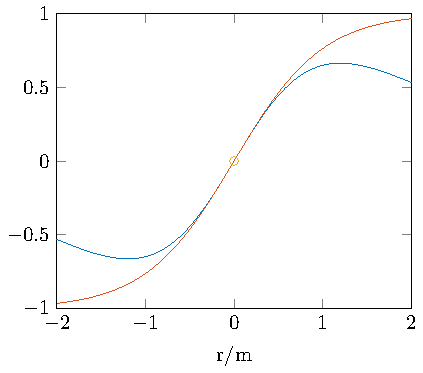
\includegraphics{./img/phase_amplitude_cond.pdf}
\caption{Plot of the holomorphy condition's two sides for the Phase-amplitude activation. $\tanh(r/m)$ is shown in red, $\text{sech}^2(r/m)(r/m)$ is shown in blue. The yellow circle indicates the point at $(0,0)$.}
\label{fig:phase_amp}
\end{figure}
This activation is holomorph at $r/m = 0$. And approximately analytic for $r/m \approx 0$ as shown in figure~\ref{fig:phase_amp}, the problem here is that this non-linearity breaks magnitude information by rescaling them, it must therefore be non-holomorph for large inputs. 

\bibliographystyle{plain}
\bibliography{literature}
\end{document}
